\documentclass[11pt]{amsart}
\usepackage{geometry}                % See geometry.pdf to learn the layout options. There are lots.
\geometry{letterpaper}                   % ... or a4paper or a5paper or ... 
%\geometry{landscape}                % Activate for for rotated page geometry
%\usepackage[parfill]{parskip}    % Activate to begin paragraphs with an empty line rather than an indent
\usepackage{graphicx}
\usepackage{amssymb}
\usepackage{epstopdf}
\usepackage [autostyle, english = american]{csquotes}
\usepackage{hyperref}
\MakeOuterQuote{"}
\DeclareGraphicsRule{.tif}{png}{.png}{`convert #1 `dirname #1`/`basename #1 .tif`.png}

\title{Project 6: Solving an Equation of Motion Using a Three Point Formula}
%\author{Jessica Bartley}
%\date{}                                           % Activate to display a given date or no date

\begin{document}
\maketitle
%\section{}
%\subsection{}

This project is about solving a second order differential equation via a "symmetric 3-point" approximation.  To my knowledge, this is not a commonly used method as there as many other ways of numerically solving differential equations.  If we so desired we could probably do this in a much more efficient / more precise way.  Nonetheless, this project seems to be asking for us to solve an equation using this three point method.  This documentation will probably change from this original write up as I'm not entirely sure  (1) what I am being asked to accomplish in this project, and (2) how to use this three point formula.
\newline

The general idea as I understand it is to estimate a derivative using the slope of the lines drawn between three points.  Say we want to take a derivative of a function but we don't know what the function is.  This is the basis for all differential equation problems.  We have some equation that involves derivatives of a function $f$ but we don't know what that $f$ is.  Say the cosine curve in Fig. 1 is our $f$ that we do not know but want to take the derivative of.  The question is: how do we approximate the derivative of $f$.  If we have three equidistant points on a curve and we want to find the derivative of the curve at the middle point then we can approximate the derivative by taking the average of each of these three slopes, drawn in light purple in Fig 1.
\newline

\begin{figure}[ht!]
\centering
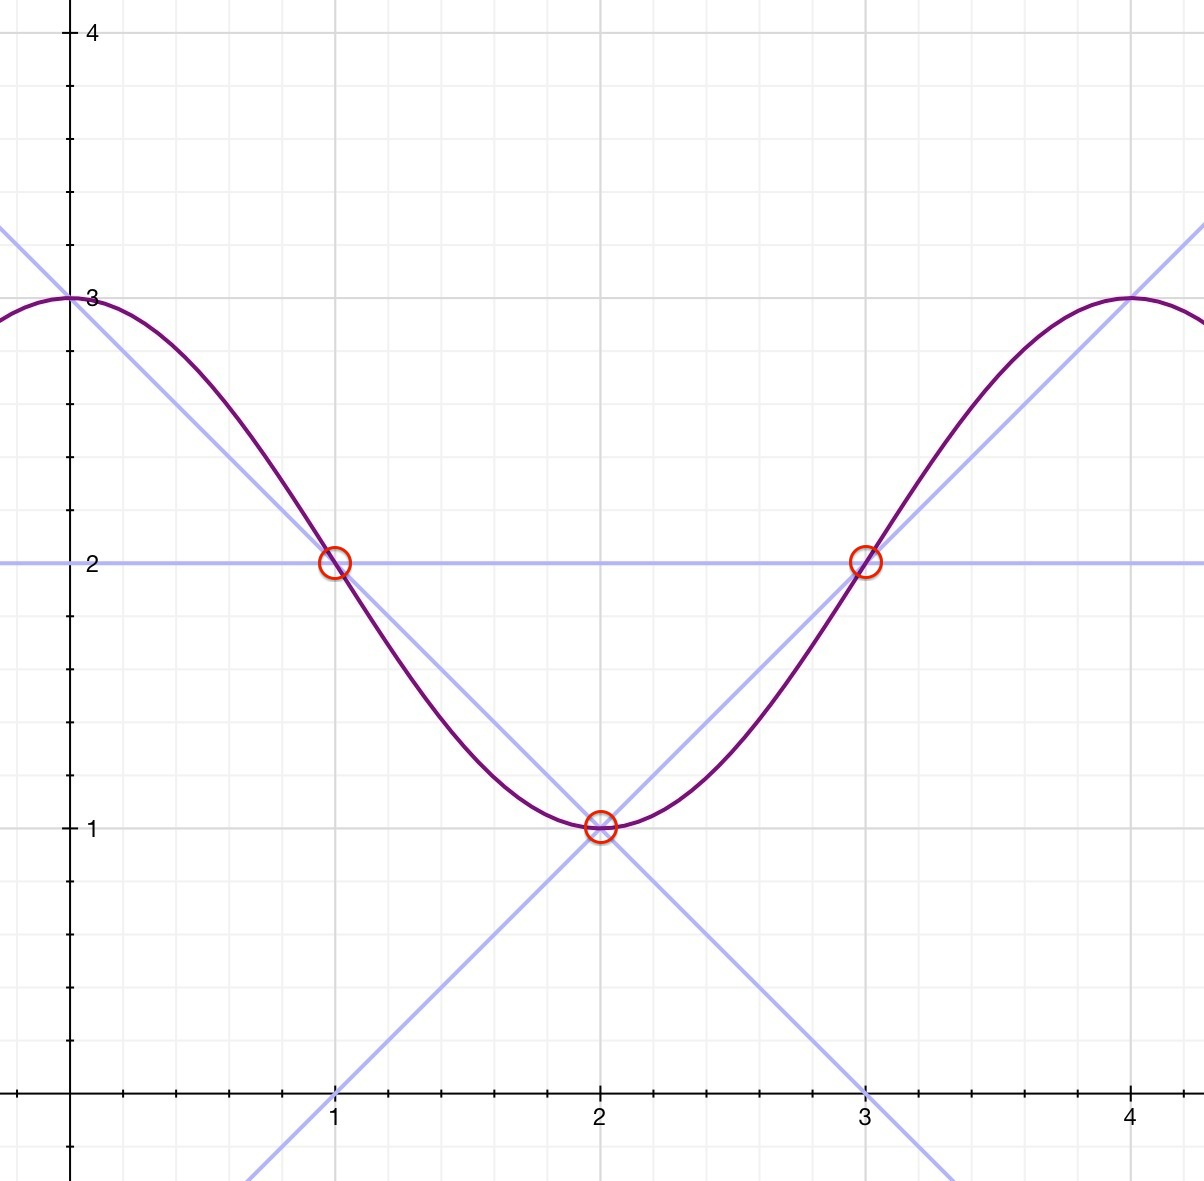
\includegraphics[width=100mm]{threepointapprox.jpg}
\caption{Three Point Approximation For the Derivative}
\label{overflow}
\end{figure}

\vspace{3 mm}

For this project we want to solve the equation of motion of a harmonic oscillator that is driven by some torque.  This equation of motion is:

\begin{equation}
\frac{d^{2} \theta}{d t^{2}} + \sin{\theta} = a \cos{\omega t}
\end{equation}
\vspace{2 mm}

First, we rewrite this second order differential equation as two first order coupled differential equations using the substitutions $x=t$, $y_1 = \theta$, and $y_2 = \frac{d \theta}{d t}$:

\begin{equation}
\frac{d y_1}{dt} = y_2
\end{equation}
\begin{equation}
\frac{d y_2}{dt} = a \cos{\omega t}- \sin{y_1}
\end{equation}

\vspace{2 mm}

Then we apply the three point formula to both of these derivatives.  We will call the first $f_1$ and the second $f_2$.  The general formula (which we will have to apply for each of $f_1$ and $f_2$) for the first derivative using the three-point method is:
\newline

\begin{equation}
f \prime (x_0) = \frac{f(x_0 + h) - f(x_0 - h)}{2h}
\end{equation}

Where $x_0$ is the middle point of interest and $h$ is the distance between points.

\end{document}  